% Annexes B, C, F et G du mémoire, archivées (décision D-20 du 2026-11-14) pour tenir le volume.
% Ce fichier n'est pas compilé avec main.tex ; il conserve le texte des annexes tel qu'il figurait dans le mémoire.
% Version compilée : memoire/main.pdf à l'étiquette v1.5 du dépôt.

\section*{Annexe B : Détail du calcul de l'ELBO pour le GMM bayésien}
\addcontentsline{toc}{section}{Annexe B : Détail du calcul de l'ELBO pour le GMM bayésien}
Cette annexe donne l'implémentation, en PyTorch, du calcul exact de l'ELBO de l'équation~\eqref{eq:1_31}~\cite[éq.~10.70 à 10.77]{bishop2006}. Les sept termes sont : $\mathbb{E}[\log p(X|Z,\mu ,\Lambda )]$, $\mathbb{E}[\log p(Z|\pi )]$, $\mathbb{E}[\log p(\pi )]$ et $\mathbb{E}[\log p(\mu ,\Lambda )]$ (partie vraisemblance et priors), puis $-\mathbb{E}[\log q(Z)]$, $-\mathbb{E}[\log q(\pi )]$ et $-\mathbb{E}[\log q(\mu ,\Lambda )]$ (entropies des facteurs variationnels). La fonction \texttt{\_ln\_B} calcule la constante de normalisation de la loi de Wishart ; \texttt{\_attendus} calcule $\mathbb{E}[\log |\Lambda _{k}|]$ (équation~\ref{eq:1_29}).

\begin{lstlisting}[language=Python]
def _ln_B(W, nu, D):
    """log de la constante de normalisation de la Wishart, ln B(W, nu)."""
    i = torch.arange(1, D + 1, dtype=torch.float64)
    lg = torch.lgamma((nu[..., None] + 1 - i) / 2).sum(-1)
    return -0.5 * nu * torch.logdet(W) - (0.5 * nu * D * LN2 + D * (D - 1) / 4 * LNPI + lg)

def _attendus(P, D):
    """E[ln|Lambda_k|] (1.29) et E[Lambda_k] pour chaque composante."""
    if P["cov_type"] in ("full", "tied"):
        i = torch.arange(1, D + 1, dtype=torch.float64)
        Elogdet = (torch.special.digamma((P["nu"][:, None] + 1 - i) / 2).sum(-1)
                   + D * LN2 + torch.logdet(P["W"]))
        Elam = P["nu"][:, None, None] * P["W"]
    else:
        psi = torch.special.digamma(P["a"]) - torch.log(P["b"])
        Elogdet = psi.sum(-1)
        Elam = torch.diag_embed(P["a"] / P["b"])
    return Elogdet, Elam

def elbo_gmm_bayesien(r, Nk, xbar, Sk, P, pr: PrioriNW):
    """
    ELBO du GMM bayésien (équation 1.31, détail dans Bishop 2006, éq. 10.70 à 10.77).
    Disponible pour la covariance pleine.
    """
    K, D = xbar.shape
    alpha, beta, m, nu, W = P["alpha"], P["beta"], P["m"], P["nu"], P["W"]
    Elogpi = torch.special.digamma(alpha) - torch.special.digamma(alpha.sum())
    Elogdet, _ = _attendus(P, D)
    dm = xbar - m
    t_trace = torch.einsum("kde,ked->k", Sk, W)
    t_quad = torch.einsum("kd,kde,ke->k", dm, W, dm)
    e_x = 0.5 * (Nk * (Elogdet - D / beta - nu * t_trace - nu * t_quad - D * LOG2PI)).sum()
    e_z = (Nk * Elogpi).sum()
    a0 = pr.alpha0
    ln_c0 = math.lgamma(K * a0) - K * math.lgamma(a0)
    e_pi = ln_c0 + (a0 - 1.0) * Elogpi.sum()
    W0 = torch.linalg.inv(pr.W0inv)
    d0 = m - pr.m0
    quad_m = torch.einsum("kd,kde,ke->k", d0, W, d0)
    nu0_t = torch.tensor(pr.nu0)
    lnB0 = _ln_B(W0, nu0_t, D)
    e_muLam = (0.5 * (D * math.log(pr.beta0 / (2 * math.pi)) + Elogdet - D * pr.beta0 / beta
                      - pr.beta0 * nu * quad_m).sum()
               + K * lnB0 + 0.5 * (pr.nu0 - D - 1) * Elogdet.sum()
               - 0.5 * (nu * torch.einsum("de,ked->k", pr.W0inv, W)).sum())
    q_z = torch.xlogy(r, r).sum()
    ln_c = torch.lgamma(alpha.sum()) - torch.lgamma(alpha).sum()
    q_pi = ((alpha - 1.0) * Elogpi).sum() + ln_c
    H = -_ln_B(W, nu, D) - 0.5 * (nu - D - 1) * Elogdet + 0.5 * nu * D
    q_muLam = (0.5 * Elogdet + 0.5 * D * torch.log(beta / (2 * math.pi)) - 0.5 * D - H).sum()
    return float(e_x + e_z + e_pi + e_muLam - q_z - q_pi - q_muLam)
\end{lstlisting}
\begin{center}\small\emph{Extrait de code : calcul de l'ELBO du GMM bayésien (équation~\ref{eq:1_31})}\end{center}

\section*{Annexe C : Table de correspondance des symboles mathématiques}
\addcontentsline{toc}{section}{Annexe C : Table de correspondance des symboles mathématiques}
Le tableau ci-dessous rappelle la signification des principaux symboles mathématiques employés dans ce mémoire, à des fins de référence rapide.

\begin{table}[H]
\centering
\small
\setlength{\tabcolsep}{0.14cm}
\begin{tabular}{|p{7.42cm}|p{7.42cm}|}
\hline
\textbf{Symbole} & \textbf{Signification} \\
\hline
X = \{$x_{1}$,\ldots{},$x_{N}$\} & Observations (données) \\
\hline
Z = \{$z_{1}$,\ldots{},$z_{N}$\} & Variables latentes \\
\hline
$\theta $ & Paramètres du modèle \\
\hline
K & Nombre de composantes du mélange \\
\hline
$\pi _{k}$ & Poids de la composante k \\
\hline
$\mu _{k}$, $\Sigma _{k}$ & Moyenne et covariance de la composante k \\
\hline
$r_{ik}$ & Responsabilité de la composante k pour l'observation i \\
\hline
$\ell $($\theta $) & Log-vraisemblance incomplète \\
\hline
Q($\theta $|$\theta ^{t}$) & Espérance de la log-vraisemblance complète \\
\hline
ELBO(q,$\theta $) & Borne inférieure de l'évidence \\
\hline
KL[$q\Vert p$] & Divergence de Kullback-Leibler \\
\hline
q($\theta $,Z) & Distribution variationnelle \\
\hline
$\alpha _{0}$, $m_{0}$, $\beta _{0}$, $W_{0}$, $\nu _{0}$ & Hyperparamètres des priors (Dirichlet, Normal-Wishart) \\
\hline
$\psi $($\cdot $) & Fonction digamma \\
\hline
$N_{k}$ & Nombre effectif de points assignés à la composante k \\
\hline
\end{tabular}
\end{table}
\section*{Annexe F : Rappels mathématiques utilisés dans les dérivations}
\addcontentsline{toc}{section}{Annexe F : Rappels mathématiques utilisés dans les dérivations}
Cette annexe rassemble, à des fins de référence, les principales définitions et identités de calcul matriciel et de statistique bayésienne mobilisées dans les dérivations du chapitre~\ref{chap:fondements} (sections~\ref{sec:formulation_mathematique_complete}.d et \ref{sec:formulation_de_l_em_variationnel}.c) et de la section~\ref{sec:de_l_energie_libre_de}, afin que le mémoire reste autonome et ne nécessite pas de recherche bibliographique complémentaire pour en suivre le détail des calculs.

\subsection*{F.1 Identités de calcul matriciel}
\textbf{Dérivée du logarithme d'un déterminant. }Pour une matrice symétrique définie positive A, on a $\partial $/$\partial A$ log|A| = ($A^{-1}$)$^{T}$ = $A^{-1}$ (la dernière égalité utilisant la symétrie de A). Cette identité est utilisée à la section~\ref{sec:formulation_mathematique_complete}.d pour dériver la mise à jour de la covariance $\Sigma _{k}$.

\textbf{Dérivée d'une forme quadratique. }Pour un vecteur x et une matrice symétrique A, on a $\partial $/$\partial A$ ($x^{T}Ax$) = $xx^{T}$. Combinée à l'identité précédente, cette formule permet d'annuler le gradient de la fonction Q par rapport à la matrice de précision $\Sigma _{k}^{-1}$, comme détaillé à la section~\ref{sec:formulation_mathematique_complete}.d.

\textbf{Trace et forme quadratique. }Pour tout vecteur x et toute matrice A, la forme quadratique $x^{T}Ax$ peut se réécrire comme une trace : $x^{T}Ax$ = tr($Axx^{T}$) = tr(A $xx^{T}$), ce qui permet de faire commuter certains calculs d'espérance avec l'opérateur trace : une manipulation fréquente, non utilisée explicitement dans les dérivations du chapitre~\ref{chap:fondements}, mais standard dans la littérature de l'inférence variationnelle pour les modèles gaussiens.

\subsection*{F.2 La distribution de Wishart}
La distribution de Wishart $\mathcal{W}$(W, $\nu $), utilisée à la section~\ref{sec:formulation_de_l_em_variationnel} comme composante du prior Normal-Wishart sur la matrice de précision $\Lambda _{k}$, généralise la distribution du $\chi ^{2}$ à des matrices. Sa densité, pour une matrice symétrique définie positive $\Lambda $ de dimension $D\times D$, est proportionnelle à :

\begin{equation}
\begin{adjustbox}{max width=0.92\linewidth}$\displaystyle \mathcal{W}(\Lambda | W{,} \nu ) \propto |\Lambda |^{(\nu -D-1)/2} \exp [-\tfrac{1}{2} \tr (W^{-1}\Lambda )]$\end{adjustbox}
\tag{F.1}
\label{eq:G_1}
\end{equation}
où W est la matrice d'échelle ($D\times D$, symétrique définie positive) et $\nu $ > D - 1 le nombre de degrés de liberté. L'espérance de cette distribution vaut $\mathbb{E}$[$\Lambda $] = $\nu W$, et l'espérance de son logarithme de déterminant, utilisée à l'équation de la section~\ref{sec:formulation_de_l_em_variationnel}.e, s'exprime au moyen de la fonction digamma multivariée : $\mathbb{E}$[log|$\Lambda $|] = $\Sigma _{j=1}^{D}$ $\psi $[($\nu $+1-j)/2] + D log 2 + log|W|, formule qui se déduit de la fonction génératrice des moments de la distribution de Wishart.

\subsection*{F.3 La distribution de Dirichlet}
La distribution de Dirichlet Dir($\alpha _{1}$, \ldots{}, $\alpha_{K}$), utilisée à la section~\ref{sec:le_theoreme_de_bayes_et} comme prior sur les poids de mélange, est la généralisation multivariée de la distribution Bêta au simplexe de dimension K-1. Sa densité s'écrit p($\pi $ | $\alpha $) $\propto $ $\prod _{k}$ $\pi _{k}^{\alpha _{k}-1}$, sous la contrainte $\sum_{k}$ $\pi _{k}$ = 1, $\pi _{k}$ $\geq $ 0. Son espérance vaut :

\begin{equation}
\begin{adjustbox}{max width=0.92\linewidth}$\displaystyle \mathbb{E}[\pi _{k}] = \alpha _{k} / \sum_{j} \alpha _{j}$\end{adjustbox}
\tag{F.2}
\label{eq:G_2}
\end{equation}
et l'espérance de son logarithme (utilisée à l'équation de la section~\ref{sec:formulation_de_l_em_variationnel}.e) s'exprime, comme pour la Wishart, au moyen de la fonction digamma : $\mathbb{E}$[log $\pi _{k}$] = $\psi $($\alpha _{k}$) - $\psi $($\sum_{j}$ $\alpha _{j}$). Cette formule intervient dans l'étape E variationnelle (équation~\ref{eq:1_27}) ; l'exemple de la section~\ref{sec:exemple_numerique_illustratif_conjugaison_dirichlet}, avec $\alpha $ = (8, 5, 2), n'en utilise que l'espérance $\mathbb{E}$[$\pi _{k}$] = $\alpha _{k}$ / $\sum_{j}$ $\alpha _{j}$.

\subsection*{F.4 La fonction digamma}
La fonction digamma $\psi $(x) = d/dx log $\Gamma $(x), dérivée logarithmique de la fonction Gamma, apparaît systématiquement dans les espérances de logarithmes de variables aléatoires des familles Dirichlet, Wishart et Gamma, en raison de la forme exponentielle de la famille exponentielle sous-jacente à ces distributions. Elle ne possède pas de forme fermée élémentaire, mais admet le développement asymptotique $\psi $(x) $\approx $ log(x) - 1/(2x) pour x grand, et est implémentée numériquement dans torch.special.digamma, utilisée dans l'implémentation de l'EM variationnel (section~\ref{sec:impl_vb}) : le code n'utilise ni SciPy ni NumPy.

\section*{Annexe G : Exemples numériques}
\addcontentsline{toc}{section}{Annexe G : Exemples numériques}
Cette annexe reprend les exemples numériques du chapitre~\ref{chap:fondements}.
\setcounter{subsection}{0}\renewcommand{\thesubsection}{G.\arabic{subsection}}\renewcommand{\theHsubsection}{G.\arabic{subsection}}
\setcounter{table}{0}\renewcommand{\thetable}{G.\arabic{table}}\renewcommand{\theHtable}{G.\arabic{table}}
\setcounter{figure}{0}\renewcommand{\thefigure}{G.\arabic{figure}}\renewcommand{\theHfigure}{G.\arabic{figure}}

\subsection{Exemple numérique : évaluation de la densité d'un GMM}\label{sec:exemple_numerique_evaluation_de_la}
Afin de rendre pleinement concrète l'équation~\eqref{eq:1_8} avant son utilisation intensive au chapitre~\ref{chap:fondements}, évaluons-la numériquement en reprenant le modèle à deux composantes convergé à la section~\ref{sec:application_au_melange_gaussien_exemple} ($\pi _{1}$=$\pi _{2}$=0,5 ; $\mu _{1}$=1,125, $\sigma _{1}$=0,466 ; $\mu _{2}$=7,725, $\sigma _{2}$=0,460), et calculons la densité prédite p(x|$\theta $) pour une nouvelle observation x = 2,0, non présente dans l'échantillon original.

\begin{equation}
\begin{adjustbox}{max width=0.92\linewidth}$\displaystyle p(2{,}0 | \theta ) = 0{,}5 \times \mathcal{N}(2{,}0 | 1{,}125 ; 0{,}466^{2}) + 0{,}5 \times \mathcal{N}(2{,}0 | 7{,}725 ; 0{,}460^{2})$\end{adjustbox}
\tag{1.10}
\label{eq:1_10}
\end{equation}
Le premier terme, associé à la composante centrée en 1,125, vaut 0,5 $\times $ 0,1468 $\approx $ 0,0734, la valeur x = 2,0 n'étant qu'à 1,9 écart-type environ du centre de cette composante. Le second terme, associé à la composante centrée en 7,725, vaut quant à lui environ 10$^{-34}$ : la valeur x = 2,0 se trouve à plus de douze écarts-types du centre de cette seconde composante, ce qui rend sa contribution totalement négligeable en comparaison de la première, un exemple numérique direct du phénomène d'underflow évoqué à la section~\ref{sec:formulation_mathematique_complete}.e, qui justifie le recours systématique au calcul en log-espace. La densité totale vaut donc p(2,0|$\theta $) $\approx $ 0,0734, et la responsabilité de la première composante pour cette observation, calculée par l'équation~\eqref{eq:1_15}, vaut $r_{1}$ = 0,0734/0,0734 $\approx $ 1,000 : le modèle attribue, sans la moindre ambiguïté, l'observation x = 2,0 à la composante centrée en 1,125, ce qui correspond parfaitement à l'intuition géométrique.

\subsection{Exemple numérique illustratif : conjugaison Dirichlet--Catégorielle}\label{sec:exemple_numerique_illustratif_conjugaison_dirichlet}
Afin d'ancrer concrètement la notion de conjugaison avant son utilisation intensive à la section~\ref{sec:em_variationnel}, illustrons-la sur le cas le plus simple rencontré dans ce mémoire : la mise à jour d'un prior de Dirichlet sur les poids d'un mélange à partir d'observations catégorielles. Considérons un mélange à K = 3 composantes, muni d'un prior a priori peu informatif Dir($\alpha _{0}$, $\alpha _{0}$, $\alpha _{0}$) avec $\alpha _{0}$ = 1 (ce qui correspond à une distribution uniforme sur le simplexe des poids $\pi $). Supposons que l'étape E d'une itération donnée attribue, sur un petit jeu de N = 12 observations, les responsabilités suivantes, cumulées par composante : $N_{1}$ = 7, $N_{2}$ = 4, $N_{3}$ = 1 (soit $\sum_{k}$ $N_{k}$ = 12, conformément à la contrainte $\sum_{k}$ $r_{ik}$ = 1 pour chaque observation).

La règle de mise à jour bayésienne pour le couple conjugué Dirichlet--Catégorielle, appliquée à la section~\ref{sec:formulation_de_l_em_variationnel}.c, donne directement le paramètre a posteriori $\alpha _{k}$ = $\alpha _{0}$ + $N_{k}$, soit ici :

\begin{equation}
\begin{adjustbox}{max width=0.92\linewidth}$\displaystyle \alpha _{1} = 1 + 7 = 8{,} \alpha _{2} = 1 + 4 = 5{,} \alpha _{3} = 1 + 1 = 2$\end{adjustbox}
\tag{1.12}
\label{eq:1_12}
\end{equation}
La distribution a posteriori sur les poids de mélange est donc Dir(8, 5, 2), dont la moyenne (l'estimation ponctuelle bayésienne des poids) vaut $\mathbb{E}$[$\pi _{k}$] = $\alpha _{k}$ / $\sum_{j}$ $\alpha _{j}$, soit $\mathbb{E}$[$\pi _{1}$] = 8/15 $\approx $ 0,533, $\mathbb{E}$[$\pi _{2}$] = 5/15 $\approx $ 0,333 et $\mathbb{E}$[$\pi _{3}$] = 2/15 $\approx $ 0,133. On notera que ces valeurs moyennes sont très proches, mais non identiques, des fréquences empiriques $N_{k}$/N = 7/12 $\approx $ 0,583 ; 4/12 $\approx $ 0,333 ; 1/12 $\approx $ 0,083 qu'aurait directement utilisées l'EM classique à l'équation~\eqref{eq:1_16} : l'écart entre les deux, plus marqué pour la composante la moins représentée (0,133 contre 0,083 pour $\pi _{3}$), illustre précisément l'effet de régularisation du prior décrit à la section~\ref{sec:avantages_de_l_em_variationnel} : le prior « tire » les estimations vers l'uniformité a priori (1/3 pour chaque composante), d'autant plus fortement que le nombre d'observations disponibles pour cette composante est faible. Cet exemple, volontairement simplifié à une seule mise à jour, préfigure directement le mécanisme itératif complet de l'EM variationnel détaillé à la section~\ref{sec:formulation_de_l_em_variationnel}, dans lequel cette même règle de mise à jour est appliquée de façon répétée, conjointement à la mise à jour des paramètres Normal-Wishart, jusqu'à convergence de l'ELBO. Ce calcul porte sur $\mathbb{E}[\pi_k]$ ; il ne doit pas être confondu avec le mécanisme d'élagage, qui repose sur $\mathbb{E}[\log \pi_k] = \psi(\alpha_k) - \psi(\sum_j \alpha_j)$ (section~\ref{sec:elagage}).

\subsection{Application au mélange gaussien : exemple numérique détaillé}\label{sec:application_au_melange_gaussien_exemple}
Afin d'illustrer concrètement le fonctionnement de l'algorithme EM classique, considérons N = 8 observations scalaires : X = \{0,5 ; 1,0 ; 1,2 ; 1,8 ; 7,1 ; 7,5 ; 8,0 ; 8,3\}. Nous supposons K = 2 composantes gaussiennes, avec pour initialisation $\mu _{1}^{0}$ = 2, $\mu _{2}^{0}$ = 6, $\sigma _{1}^{0}$ = $\sigma _{2}^{0}$ = 2, $\pi _{1}^{0}$ = $\pi _{2}^{0}$ = 0,5. Le tableau~\ref{tab:t1_2} retrace l'évolution des paramètres au fil des itérations ; la log-vraisemblance indiquée est celle des paramètres obtenus à l'issue de l'étape M de l'itération considérée.

\tableauGenere{t1_2}
La convergence est très rapide : le point fixe est atteint en trois itérations, la variation de la log-vraisemblance devenant inférieure à $10^{-3}$ dès l'itération suivante. La log-vraisemblance croît de -15,814 à -10,736 sans jamais diminuer, conformément à la garantie théorique établie précédemment. La solution finale identifie correctement les deux groupes : le premier est centré sur 1,125 (moyenne empirique des observations 0,5 ; 1,0 ; 1,2 et 1,8) avec un écart-type de 0,466, le second sur 7,725 (moyenne empirique de 7,1 ; 7,5 ; 8,0 et 8,3) avec un écart-type de 0,460. Les deux groupes étant très éloignés l'un de l'autre, les responsabilités valent 1 ou 0 à la précision de la machine et les paramètres estimés coïncident avec les statistiques empiriques de chaque groupe.

\begin{figure}[H]
\centering
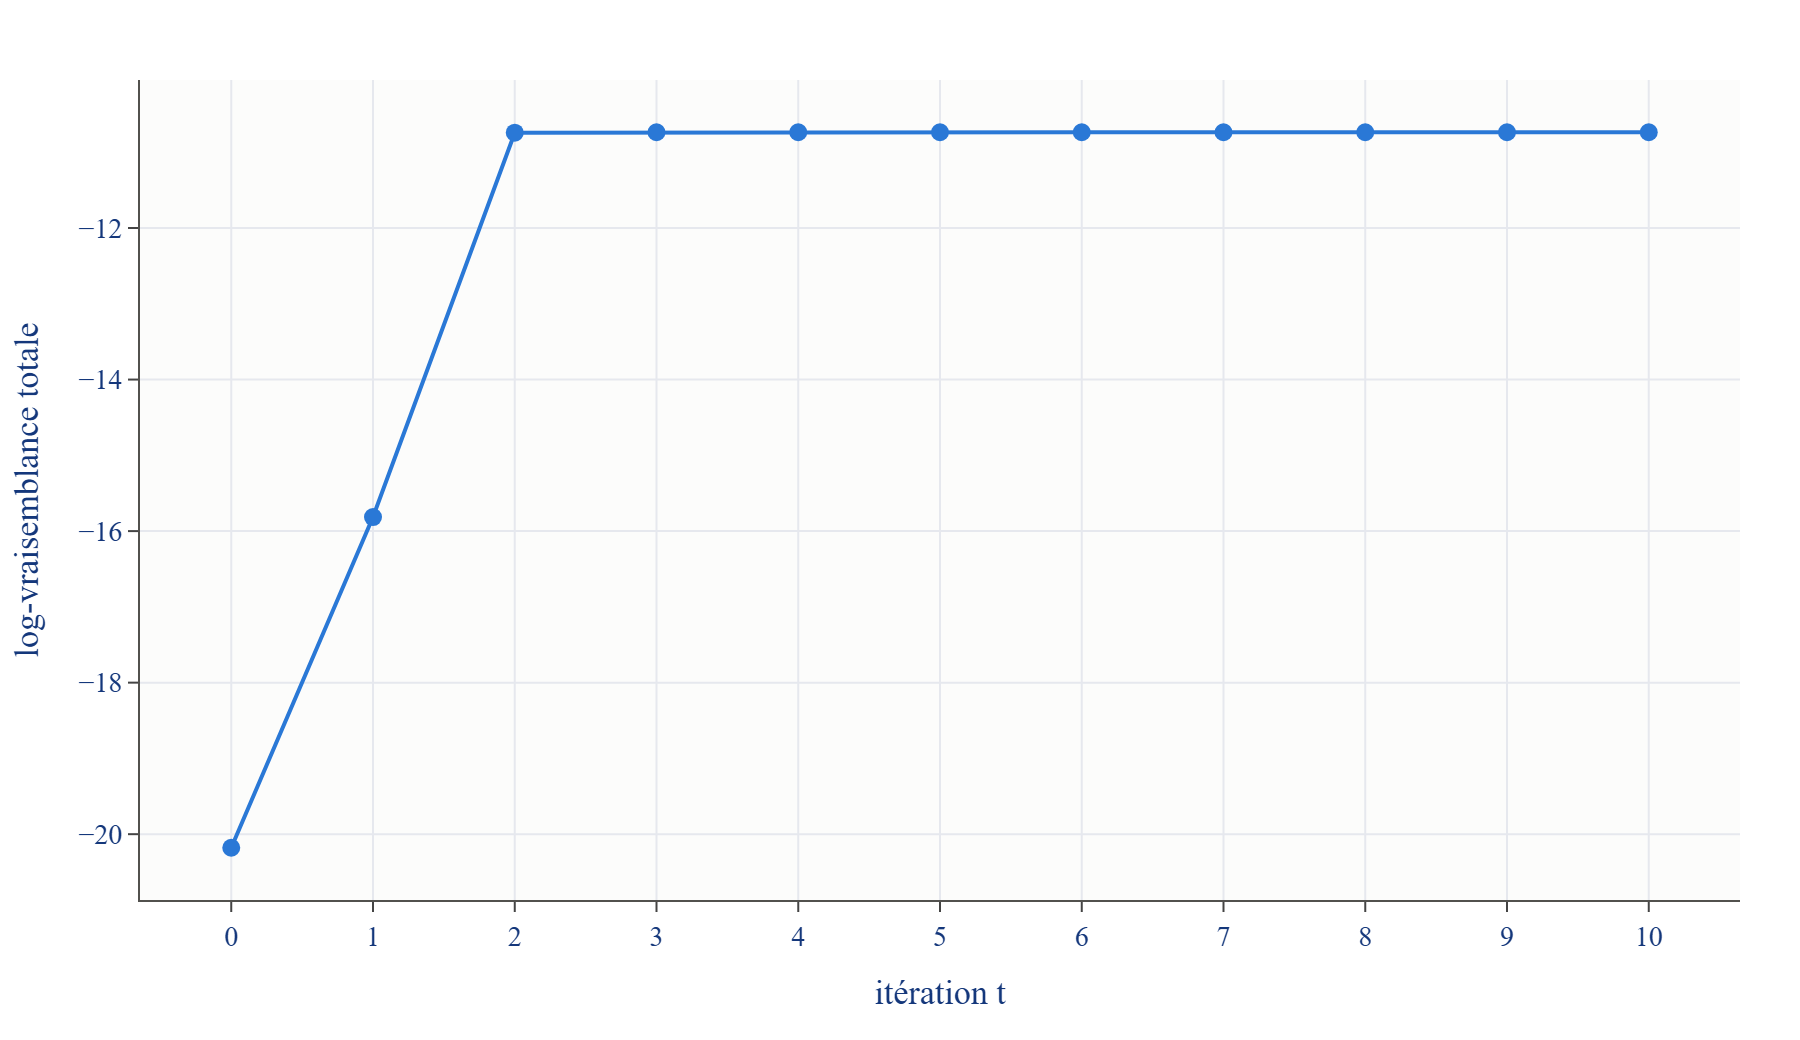
\includegraphics[width=0.85\textwidth]{figures/fig01.png}
\caption{Évolution de la log-vraisemblance au fil des itérations (exemple numérique de la section~\ref{sec:application_au_melange_gaussien_exemple}). La courbe est croissante puis stationnaire dès la troisième itération, ce qui illustre la garantie de monotonie établie à la section~\ref{sec:formulation_mathematique_complete}.f.}
\label{fig:1_1}
\end{figure}

\subsection{Exemple numérique illustratif}\label{sec:exemple_numerique_illustratif}
Afin de rendre plus concret le mécanisme d'élagage décrit à la section~\ref{sec:elagage}, reprenons l'exemple numérique de la section~\ref{sec:application_au_melange_gaussien_exemple} : les huit observations scalaires X = \{0,5 ; 1,0 ; 1,2 ; 1,8 ; 7,1 ; 7,5 ; 8,0 ; 8,3\}, qui forment visiblement deux groupes bien séparés. Appliquons cette fois l'EM variationnel avec $K_{\max} = 3$ composantes (soit une de plus que le nombre réel de groupes), un prior de Dirichlet de concentration $\alpha _{0}$ = 1/3, et des priors Normal-Wishart non informatifs ($\beta _{0}$ = 10$^{-3}$, $\nu _{0}$ = 1, $W_{0}$ = 1).

L'algorithme converge en 5 à 15 itérations selon l'initialisation (critère $|\Delta \mathrm{ELBO}| < 10^{-6}$), vers la même solution dans les dix essais réalisés (graines 0 à 4, initialisation par les hyperparamètres ou par k-means). Le tableau~\ref{tab:t1_5} présente les paramètres finaux obtenus pour chacune des trois composantes.

\tableauGenere{t1_5}
Ce résultat illustre de façon particulièrement nette le mécanisme théorique décrit à la section~\ref{sec:elagage}. Les deux premières composantes se partagent presque également la masse de probabilité (poids 0,482 chacune), avec des moyennes de 7,724 et 1,126 qui coïncident, à $10^{-3}$ près, avec les moyennes empiriques des deux groupes et avec la solution de l'EM classique de la section~\ref{sec:application_au_melange_gaussien_exemple} (7,725 et 1,125). La troisième composante, en revanche, voit son paramètre $\alpha _{k}$ rester exactement égal à sa valeur initiale $\alpha _{0}$ = 1/3 = 0,333, signe que $N_{k}$ = $\alpha _{k}$ - $\alpha _{0}$ = 0 : aucune observation, même partiellement, ne lui a été attribuée au cours de la convergence. Cette composante est donc entièrement inactive, et le modèle retient effectivement $K_{\text{effectif}}$ = 2 composantes actives, exactement le nombre réel de groupes : un résultat que l'EM classique, avec K fixé à l'avance, ne peut pas produire de lui-même : il faudrait, pour l'EM classique, comparer explicitement les solutions à K = 2 et K = 3 au moyen d'un critère externe tel que le BIC, alors que l'EM variationnel effectue cette sélection de façon endogène, en une seule exécution.

